\pdfminorversion=4
\documentclass[mathserif,xcolor={dvipsnames,table}]{beamer}
\mode<presentation>{\usetheme{Warsaw}\usecolortheme{crane}}
\usepackage{centernot}
\usepackage{graphicx}
\usepackage{geometry}
\usepackage{upgreek}
\usepackage{lipsum}
\usepackage{cutwin}
\usepackage{tikz}
\usetikzlibrary{shadows}
\usepackage[utf8]{inputenc}
\usepackage[english]{babel}
\usepackage[T1]{fontenc}
\usepackage{lmodern}
\usepackage[babel=true]{microtype}
\beamertemplatenavigationsymbolsempty

\title{\textbf{Your Friend the Computer \\(aka Computer Architecture)}}
\date{}
\author{CS4803UWS at the\\
Georgia Institute of Technology
}

\begin{document}

\begin{frame}
\titlepage
\begin{center}

\includegraphics[scale=0.33]{images/uws.png}\\
\vspace{.1in}
\tiny{copyright \copyright\ 2013}\\

\includegraphics[scale=.25]{images/cc-logo.pdf}

\includegraphics[scale=.25]{images/cc-new.pdf}

\includegraphics[scale=.25]{images/cc-share.pdf}\\
\tiny{creative commons 3.0 share-alike attribution license}
\end{center}
\end{frame}

\begin{frame}{The purpose of a systems programmer}
\textbf{Given system $S$, and problem $P$,\\
we will implement $P$,\\
using the resources of $S$,\\
subject to some constraint.}\\
\vspace{.25in}
That constraint is typically to minimize either:
\begin{itemize}
\vspace{.05in}
\item time to completion,
\vspace{.05in}
\item power to completion, or
\vspace{.05in}
\item $\text{time to completion}\cdot\text{utilization.}\footnote{Constrained by some minimum utilization.}$
\end{itemize}
\vspace{.25in}
Proving that these constraints have been met is clearly
dependent upon the details of both $P$ and $S$.
\end{frame}

\begin{frame}{Chasing peak}
How can we know when we're ``done''? Absolute measurements
can be taken in terms of the system's theoretical \textbf{peak} perf.\\
\vspace{.15in}
Peak is a slippery concept. What follows are my opinions:
\vspace{.15in}
\begin{itemize}
\item ``Peak'' seems most \textit{precisely} defined in terms of the ISA of $S$
(which might be irrelevant to our problem).
\item ``Peak'' seems most \textit{correctly} defined in terms of the best possible
solution to $P$ (which might be unknown).
\item ``Peak'' seems most \textit{productively} defined in terms of the instructions our actual
implementation would use in the absence of structural hazards.
\end{itemize}
\vspace{.15in}
In my experience, it is generally misleading to compare how closely
different $P$ approach their own peaks. Most often, we use ``peak'' within
the context of a small section of code.
\end{frame}

\begin{frame}{Instructions I}
Start in some initial state, and evolve in discrete timesteps
according to some primitive recursive function closed on that state.\\
\vspace{.25in}
Each time step is a \textit{cycle}(\textbf{c}). 1GHz$\implies$ 1ns \textbf{c}-time.\\
\vspace{.25in}
``Running a program'' is the act of denoting words of this state
as ``current instructions'', causing them to drive control flow.
\vspace{.25in}
\begin{itemize}
\item Static instructions: Instructions in a sequence
\item Dynamic instructions: Instructions \textit{executed} in a sequence
\item IPC: Instructions per \textbf{c}
\item CPI: \textbf{c} per instruction
\end{itemize}
\end{frame}

\begin{frame}{Instructions II}
Instructions lie at the boundary between those abstractions we \textit{control} and those
we merely \textit{exploit}.
\begin{equation}
P_{time} = Inst_{dynamic}\cdot CPI_{avg}\cdot\nu
\end{equation}
The means of accelerating our program are finite:
\begin{enumerate}
\item Reduce \textbf{c}-time (better $\upmu$architecture, better materials)
\item Require fewer instructions (better code, better algorithms, more powerful instructions, AQC)
\item Reduce CPI (better $\upmu$arch, better code, VLIW/EPIC)
\item Add time (increased high-level parallelism)
\item Dilate time (relativistic motion)
\end{enumerate}
\vspace{.1in}
\#5 is a tool of the future, and \#1 is a tool of the past.
Understanding why will require a detour into physics. Hold on tight!
\end{frame}

\begin{frame}{\textbf{c}-time}
Taken to the limit, we can 
\begin{equation}
\end{equation}
\end{frame}

\begin{frame}{Digital logic}
\tiny{\textit{Symmetric CMOS inverters} ($V_{T_{n}} = |V_{T_{p}}|$,
$C^{*}_{oxn} = C^{*}_{oxp}$, and
$K_n = K_p$ ($K_{foo,ox}\triangleq \frac{\mu_{foo}\kappa_{ox}}{2T_{ox}}$,
where $\mu = \text{electron mobility in}\ foo$,
$\kappa = \text{relative permittivity in}\ ox$,
and $T = \text{thickness of insulator oxide}\ ox$)
%$\kappa$ is frequently written $\varepsilon$ and refered to as ``dielectric constant''
draw power only while switching, maximize use of clocks, and require only 
a pMOS and nMOS transistor in series.}
\begin{figure}
\begin{center}
\fbox{\tiny{RTL}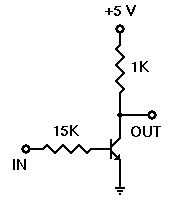
\includegraphics[height=.5in,width=0.1\textwidth]{images/rtl_inverter_sch.png}}
\fbox{\tiny{TTL}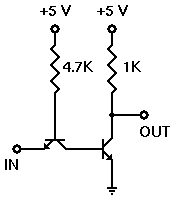
\includegraphics[height=.5in,width=0.1\textwidth]{images/ttl.png}}   
\fbox{\tiny{pMOS}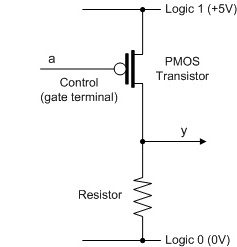
\includegraphics[height=.49in,width=0.1\textwidth]{images/pmos.jpg}}   
\fbox{\tiny{nMOS}\includegraphics[height=.5in,width=0.1\textwidth]{images/nmosinverter.pdf}}   
\fbox{\tiny{CMOS}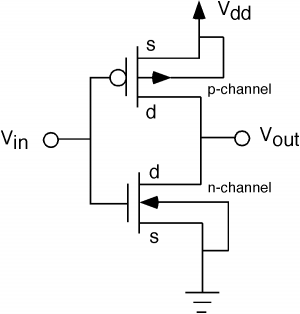
\includegraphics[height=.5in,width=0.1\textwidth]{images/cmos.png}}
\end{center}
\tiny{\textbf{Given inverters, we can build (\textit{functionally complete}) NORs and NANDs\footnote{\tiny{CMOS NOR/NAND in 4 transistors each; TTL multiemitters requires 5 for NOR vs. 4 for NAND.}}\ldots}}
\end{figure}
\begin{figure}
\begin{center}
%\fbox{\tiny{RTL}\includegraphics[height=.5in,width=0.1\textwidth]{images/rtl-npn-nor.pdf}}
%\fbox{\tiny{TTL}\includegraphics[height=.5in,width=0.1\textwidth]{images/ttlnor.png}}
\fbox{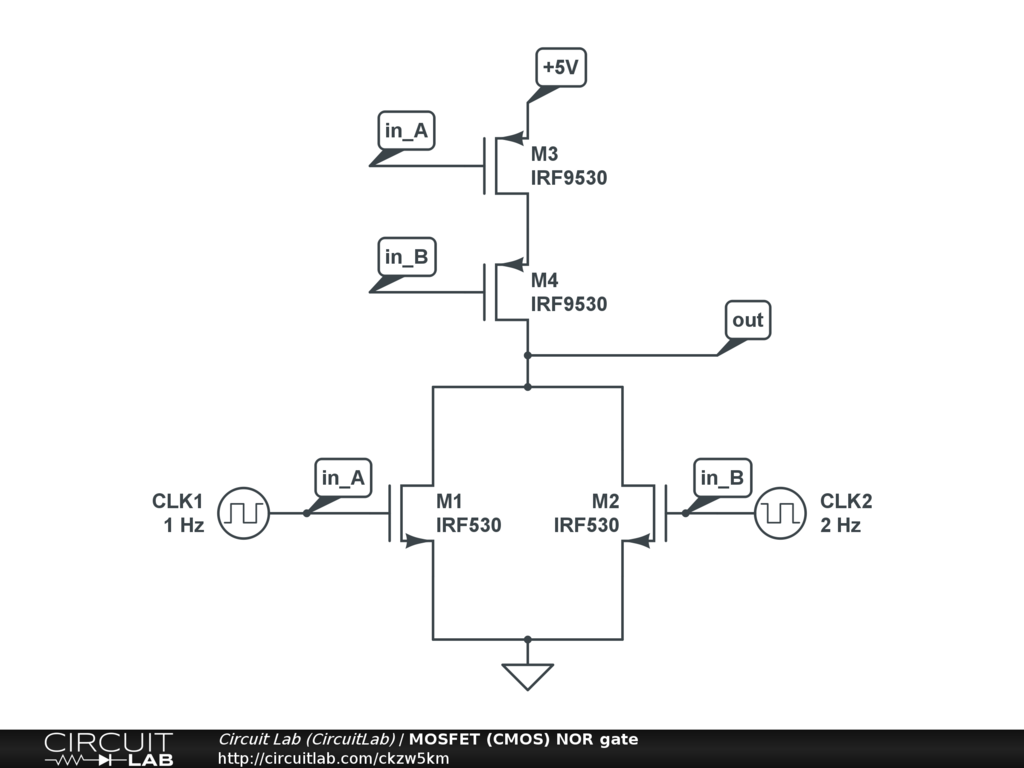
\includegraphics[width=0.25\textwidth]{images/cmosnor.png}}
\fbox{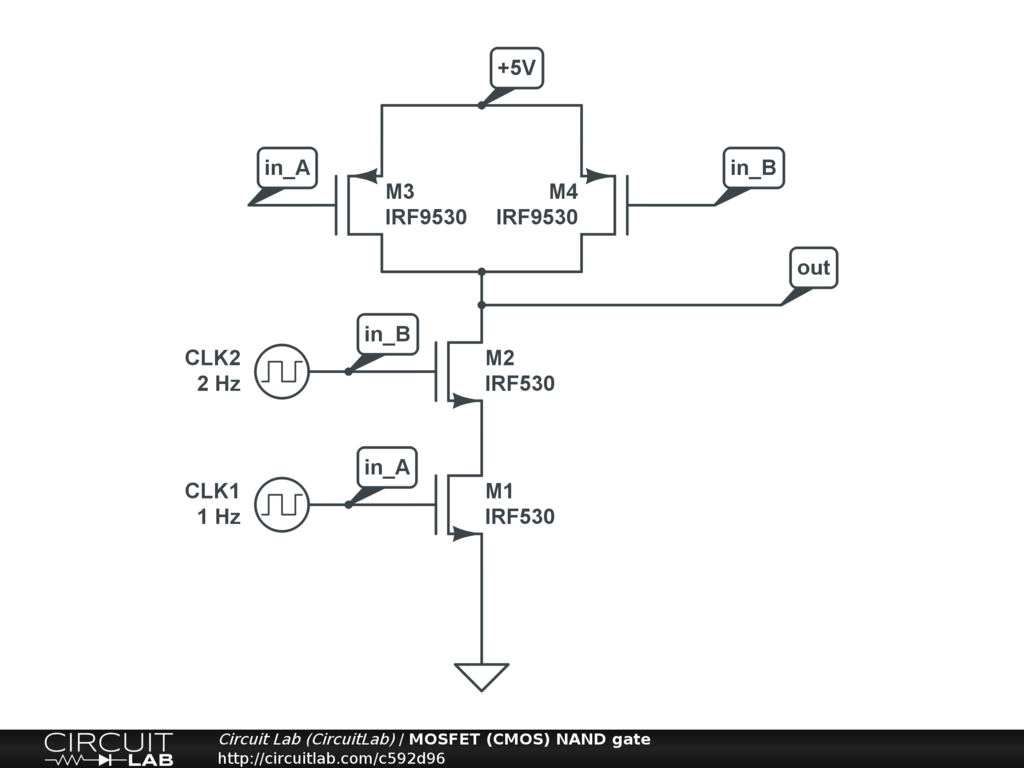
\includegraphics[width=0.25\textwidth]{images/cmosnand.png}}
\end{center}
\tiny{\textbf{\ldots given NORs and NANDs, we can build universal computers\ldots}}
\end{figure}

\begin{figure}
\begin{center}
%\fbox{\tiny{RTL}\includegraphics[height=.5in,width=0.1\textwidth]{images/rtl-npn-nor.pdf}}
%\fbox{\tiny{TTL}\includegraphics[height=.5in,width=0.1\textwidth]{images/ttlnor.png}}
\fbox{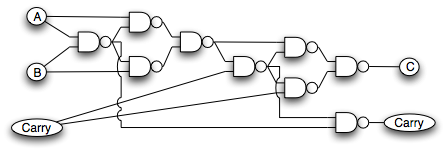
\includegraphics[width=0.25\textwidth]{images/nandadder.png}}\\
\tiny{\textbf{\ldots and \textit{now} we're getting somewhere. Delicious!}}
\end{center}
\end{figure}
\end{frame}

\begin{frame}{Complementary metal-oxide semiconductors I}
Draw \textit{greatest} power only when changing state\ldots\footnote{Though, as $\nu\rightarrow\infty$, $\frac{T_{switching}}{T_{total}}\rightarrow 1$\ldots\\}
\begin{equation}
P_{dynamic} = \alpha C_LV_{DD}^{2}\nu
\end{equation}
\begin{description}
\item[$P$] Dynamic power ($W = J/s = \frac{m^{2}\cdot kg}{s^{3}}$)
\item[$C_L$] Load capacitances ($F = \frac{A^{2}\cdot s^{4}}{m^{2}\cdot kg}$)
\item[$\alpha$] Activity factor
\item[$V_{DD}$] Supply voltage ($V = \frac{m^{2}\cdot kg}{A\cdot s^{3}}$)
\item[$\nu$] Frequency ($1/s$)
\end{description}
\vfill
\textbf{NB:} $P_{dynamic}$ increases with the \textit{square} of $V_{DD}$.
\end{frame}

\begin{frame}{Complementary metal-oxide semiconductors II}
\ldots but always consume \textit{some} power:
\begin{equation}
P_{static} = I_{static}\cdot V_{DD}
\end{equation}
\begin{description}
\item[$P$] Static power ($W = V\cdot A$)
\item[$I_{static}$] Static current ($I_{subth}\footnote{Leakage between MOS source and drain} + I_{tunnel}\footnote{Leakage across semiconductor junctions} + I_{leakage}\footnote{Leakage through the insulator}, A$)
\item[$V_{DD}$] Supply voltage ($V$)
\end{description}
\vspace{.15in}
This has become more important as transistor count has increased and sizes
have shrunk.
\vfill
\textbf{Implication:} power draw is independent of actual state.
\textbf{Implication:} for fixed work, lower $\upnu$ usually cannot
save power.
\end{frame}

\begin{frame}{Caring for and feeding your MOSFET I}
\renewcommand\windowpagestuff{%
\includegraphics[height=1.5cm,width=4cm]{images/vtf.png}
\par{\usebeamercolor[fg]{caption name}%
\usebeamerfont*{caption name}%\figurename%
\usebeamertemplate{caption label separator}}%
%\raggedright%
\usebeamerfont*{caption}%
%\tiny{CMOS inverter voltage transfer function}%
}
\opencutleft
%\begin{cutout}{0}{0cm}{.8\linewidth}{4}
{\scriptsize nMOS (``negative MOS'') uses
$e^{-}$ as charge carriers, n+ source, drain, and gate, and p-substrate. With no
mobile carriers, $I_{D_{C}} = 0$. $V^{+}_{GS}$
is applied to the gate, attracting electrons as $V_{GS}\ \text{exceeds the threshold
voltage}\ V_{TH}$, establishing a salient.
$I_{D_{TL}} = \frac{\mu_{n}C^{*}_{oxn}W}{2L}\left[2(V_{GS} - V_{TH})V_{DS} - V^{2}_{DS}\right]$, growing
linearly with $V_{GS}$. Once $V_{DSat}\triangleq V_{GS} - V_{TH} \ge V_{DS}$, a
conducting channel exists from source to drain, and $I_{DSat} = \frac{\mu_{n}C^{*}_{oxn}W}{2L}\left[V_{GS} - V_{TH}\right]^{2}$. We call these three modes \textit{cutoff},
\textit{linear}, and \textit{saturation}. This switch requires discharging the charge in our nMOSFET:\\
\begin{equation}
\tau_{pHL} \approx \frac{\text{charge on} C_L}{2 * \text{NMOS discharge current}} = \frac{L_{n}C_{L}V_{DD}}{W_{n}\mu_{n}C^{*}_{ox}\left(V_{DD} - V_{TH}\right)^{2}}
\end{equation}
Where appropriate, pMOS reverses the signs\footnote{Using holes, not $e^{+}$ (positrons).}.
}
\\
\vfill
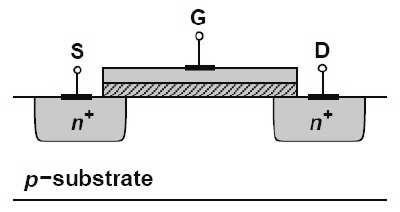
\includegraphics[scale=.3]{images/oe-001.png}
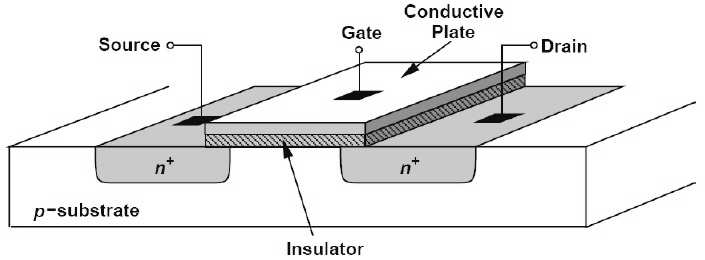
\includegraphics[scale=.3]{images/oe-000.png}
%\end{cutout}
\end{frame}

\begin{frame}{Caring for and feeding your MOSFET II}
\lipsum[1]
\end{frame}

% FIXME
% Show how this does *not* allow us to perform any operation in a single
% instruction -- SHA-1 is a map from 512B to 120B, that mixes the input in
% amongst itself, and thus would require a 512B->120B map.
\begin{frame}{Instructions III}
Fully generally, instructions map input states to output states.
\small{
\begin{itemize}
\item A machine could contain in ROM a lookup table containing every possible
function from $2^{n*\text{word}}\implies 2^{m*\text{word}}$. Each instruction
specifies inputs, outputs, and a map selection\footnote{Calculate this ROM's size, and the minimum instruction size.}.
\item A machine could allow each instruction to specify a single lookup table implementing
a single such map\footnote{Calculate the minimum necessary instruction size.}.
\item ``Arithmetic MISC'' provides universal computation via a single arithmetic instruction
operation, memory addresses, and a conditional branch target in every instruction.
\item``Transport-triggered MISC`` (sometimes called ZISC) involves memory-mapped
functional units and a branch. All MISC schemes require the ability to modify one's
own code\footnote{Prove this.}.
\end{itemize}
}
\end{frame}

\begin{frame}{Special registers}
Often read-only/privileged/require special instructions.
\tiny{
\begin{itemize}
\item $EIP$: Read-only. Instruction pointer
\item $EFLAGS$: Flags register. Contains IOPL/CPL (\texttt{POPF}/\texttt{IRET})
\item $CR_0$: Machine Status Control Word (\texttt{LMSW}, 286+)
\item $CR_2$: Read-only. Page fault addresses (386+)
\item $CR_3 (PDBR)$: Page Directory Base Reg. (386+)
\item $MXCSR$ SSE Control Status Reg. (\texttt{LD/STMXCSR}, PIII+)
\item $DR_0, DR_1, DR_2, DR_3, DR_7$: Debug Reg.
\item $CS, DS, ES, FS, GS, SS$: Segment Reg.
\item $TR$: Task Register (\texttt{LTR}/\texttt{STR})
\item $GDTR$: Global Descriptor Table Reg. (\texttt{LGDT}/\texttt{SGDT}, 286+)
\item $LDTR$: Local Descriptor Table Reg. (\texttt{LLDT}, 286+)
\item $IDTR$: Interrupt Descriptor Table Reg. (\texttt{LIDT}/\texttt{SIDT}, 286+)
\item $TPR$: Task Priority Reg.
\item $PPR$: Process Priority Reg.
\item $TSC$: Timestamp Counter (\texttt{RDTSC}, Pentium+)
\item $PMC_n$: Performance Monitoring Counters (\texttt{RDPMC}, MMX+)
\item $MSR_n$: Model-Specific Reg. (\texttt{RD/WRMSR}, Pentium+)
\end{itemize}
}
\end{frame}

\begin{frame}{General-purpose registers}
\begin{itemize}
\item Read ports pace superscalability
\item Write ports pace instruction retire
\item Register width paces bit parallelism
\item Architectural registers pace memory accesses
\item Physical registers pace OOO hiding of antidependency
% particularly useful for EFLAGS!
\end{itemize}
\end{frame}

\begin{frame}{Register file (indexed access)}
\begin{itemize}
\item Architectural registers are exposed as PRAM or a stack
\item SRAM cells + read/write lines + decoder tree + sense amps
\item One internal bit line per bit of read port
\item Two internal bit lines per bit of write port
\item One word line per entry
\item Transistor area grows linearly with number of ports
\item Wire pitch area grows with square of number of ports
\item Hence: register \textit{banking}
\end{itemize}
\end{frame}

\begin{frame}{Fundamental theorem of data starvation}
We can only hit peak during sequences of code which fully
utilize arithmetic resources. Registers must provide throughput
at least equivalent to the processor's arithmetic throughput.\footnote{\tiny{In a classic load/store RISC architecture, arithmetic instructions operate
only on registers. In a machine admitting memory addresses as inputs to
arithmetic operands, such instructions will exhibit greater latency and lesser throughput
than their register-direct counterparts (though not always; see Intel NetBurst/Core ``micro-fusion'').}}\\
\vspace{.35in}
\textbf{THUS,} a memory lacking throughput greater than or equal to the ratio of
arithmetic/register throughput to arithmetic intensity ($\textbf{c}$ per word) will not be able
to sustain peak.
\end{frame}

\begin{frame}{Sandy Bridge frontend}
The modern x86 frontend is tremendously complicated due to its inherited ISA,
yet it manages to deliver $\upmu$ops to the superscalar dataflow-ordered
execution core at full throughput. How?
\vfill
\begin{itemize}
\item 16B/\textbf{c} fetches from 32KB 8-way\footnote{4-way on Nehalem} I\$
\item Speculative decoding at each of fetch's 16B
\item 1 complex decoder, 3 simple decoders
\item 32 sets of 8 ways of 6 $\upmu$op $\upmu$I\$ (``decoded I\$'')
\item 28$\upmu$op $\upmu$L\$ (``Loop stream detector'') per thread\footnote{On HyperThreaded Ivy Bridge, 56 $\upmu$ops if one logical core is inactive.}
\item 4$\upmu$op/\textbf{c} renamer-scheduler
\item Macro- and micro-fusion
\end{itemize}
\end{frame}

\begin{frame}{Frontend delays}
\begin{itemize}
\item Instruction fetch miss (7\textbf{c} for ITLB miss + 2TLB hit)
\item 3\textbf{c} for each non-REX length changing prefix\footnote{6\textbf{c} for any fetch containing an LCP on Nehalem}
\item Instruction decode delay / MSROM access
\item \huge\textbf{FIXME}
\end{itemize}
\end{frame}

\begin{frame}
\huge FIXME talk about OOO-dataflow limit, FO4, why higher freq requires more
pipelining, etc.
\end{frame}

\begin{frame}{Why we fall short of peak}
\begin{center}
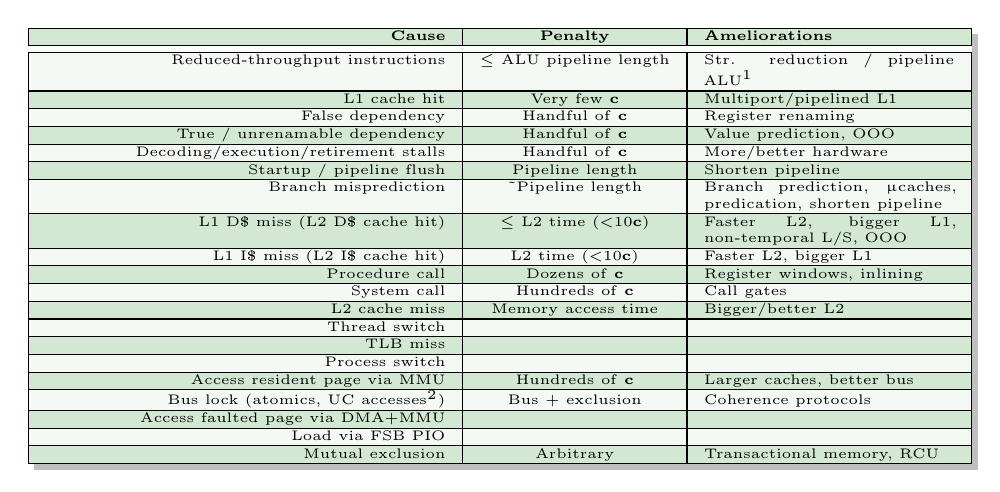
\begin{tikzpicture}
\node[drop shadow,fill=white,inner sep=0pt]
{\rowcolors{1}{ForestGreen!20}{ForestGreen!5}
{\tiny
\begin{tabular}{|>{\raggedleft}p{2in}|c|p{1.25in}|}
\hline
\textbf{Cause} & \textbf{Penalty} & \textbf{Ameliorations} \\
\hline\hline
Reduced-throughput instructions & $\le$ ALU pipeline length &
Str. reduction / pipeline ALU\footnote{Explain how lengthening the ALU pipeline
might be beneficial despite the delay being bounded by this pipeline's length.}  \\
\hline
L1 cache hit & Very few \textbf{c} & Multiport/pipelined L1 \\
\hline
False dependency & Handful of \textbf{c} & Register renaming \\
\hline
True / unrenamable dependency & Handful of \textbf{c} & Value prediction, OOO \\
\hline
Decoding/execution/retirement stalls & Handful of \textbf{c} & More/better hardware \\
\hline
Startup / pipeline flush & Pipeline length & Shorten pipeline \\
\hline
Branch misprediction & \textasciitilde Pipeline length & Branch prediction, $\upmu$caches,\linebreak predication, shorten pipeline \\
\hline
L1 D\$ miss (L2 D\$ cache hit) & $\le$ L2 time (<10\textbf{c}) & Faster L2, bigger L1,\linebreak non-temporal L/S, OOO \\
\hline
L1 I\$ miss (L2 I\$ cache hit) & L2 time (<10\textbf{c}) & Faster L2, bigger L1 \\
\hline
Procedure call & Dozens of \textbf{c} & Register windows, inlining \\
\hline
System call & Hundreds of \textbf{c} & Call gates \\
\hline
L2 cache miss & Memory access time & Bigger/better L2 \\
\hline
Thread switch & & \\
\hline
TLB miss & & \\
\hline
Process switch & & \\
\hline
Access resident page via MMU & Hundreds of \textbf{c} & Larger caches, better bus \\
\hline
Bus lock (atomics, UC accesses\footnote{Including pagewalks of uncacheable tables.}) & Bus + exclusion & Coherence protocols \\
\hline
Access faulted page via DMA+MMU & & \\
\hline
Load via FSB PIO & & \\
\hline
Mutual exclusion & Arbitrary & Transactional memory, RCU \\
\hline
\end{tabular}%
}
};
\end{tikzpicture}
\end{center}
\end{frame}

\begin{frame}{Optimization methodology\hfill\tiny{Adapted from the \textit{Intel Optimization Manual}}}
Are we hitting peak? If not, let's account for each cycle:\\
\vspace{.15in}
Are we fully utilizing the system?
\begin{itemize}
\item No. Why not?
\begin{itemize}
\item Contention among threads?
\item Blocking on I/O?
\item Incomplete exploitation of multiple processors / SIMD?
\end{itemize}
\end{itemize}
Yes. Are we issuing $\upmu$ops?
\begin{itemize}
\item No. What's causing our frontend stall?
\begin{itemize}
 \item Store-forwarding?
 \item LCP delay?
 \item Cache miss?
\end{itemize}
\end{itemize}
Yes. Are we retiring $\upmu$ops?
\begin{itemize}
 \item No. What's clogging our backend?
 \begin{itemize}
  \item Branch mispredictions?
  \item Dependency chains?
 \end{itemize}
\end{itemize}
Yes. Look for strength reduction or new algorithms.

\end{frame}

\begin{frame}{Recommended reading}
\footnotesize{
\begin{itemize}
\item Andi Kleen. ``Linux multi-core scalability'' (2009).
\item Doug Carmean and Eric Sprangle. ``Increasing Processor Performance by Implementing Deeper Pipelines'' (2002).
\item Ulrich Drepper. ``What Every Programmer Needs to Know About Memory'' (2007). Linux Weekly News, in eight parts.
\item Paul McKenney. ``Transactional Memory Everywhere'' (2012).
\item Ward and Halstead. ``Computation Structures'' (1990).
\item John Shen and Mikko Lipasti. \textit{Modern Processor Design} (2004).
\item Agner Fog. \textit{The microarchitecture of Intel, AMD and VIA CPUs: An optimization guide for assembly programmers and compiler makers} (regularly updated). http://www.agner.org.
\item Bruce Shriver and Bennett Smith. \textit{The Anatomy of a High-Performance Microprocessor: A Systems Perspective} (1998).
\item \textit{Intel 64 and IA-32 Architectures Optimization Manuals}.
\end{itemize}
}
\end{frame}

\begin{frame}{Hack on!}
``The purpose of abstraction is not to be vague, but to create a new semantic level in which one can be absolutely precise.''\\
\hfill---Edsger Dijkstra
\vfill
``The most amazing achievement of the computer software industry is its 
continuing cancellation of the steady and staggering gains made by the 
computer hardware industry.''\hfill---Henry Petroski
\vfill
\vfill
``First you learn the value of abstraction. Then you learn the cost of abstraction. Then you're ready to engineer.''\\
\hfill---Kent Beck
\end{frame}

\end{document}
